\PassOptionsToPackage{unicode=true}{hyperref} % options for packages loaded elsewhere
\PassOptionsToPackage{hyphens}{url}
%
\documentclass[
  ignorenonframetext,
]{beamer}
\usepackage{pgfpages}
\setbeamertemplate{caption}[numbered]
\setbeamertemplate{caption label separator}{: }
\setbeamercolor{caption name}{fg=normal text.fg}
\beamertemplatenavigationsymbolsempty
% Prevent slide breaks in the middle of a paragraph:
\widowpenalties 1 10000
\raggedbottom
\setbeamertemplate{part page}{
  \centering
  \begin{beamercolorbox}[sep=16pt,center]{part title}
    \usebeamerfont{part title}\insertpart\par
  \end{beamercolorbox}
}
\setbeamertemplate{section page}{
  \centering
  \begin{beamercolorbox}[sep=12pt,center]{part title}
    \usebeamerfont{section title}\insertsection\par
  \end{beamercolorbox}
}
\setbeamertemplate{subsection page}{
  \centering
  \begin{beamercolorbox}[sep=8pt,center]{part title}
    \usebeamerfont{subsection title}\insertsubsection\par
  \end{beamercolorbox}
}
\AtBeginPart{
  \frame{\partpage}
}
\AtBeginSection{
  \ifbibliography
  \else
    \frame{\sectionpage}
  \fi
}
\AtBeginSubsection{
  \frame{\subsectionpage}
}
\usepackage{lmodern}
\usepackage{amssymb,amsmath}
\usepackage{ifxetex,ifluatex}
\ifnum 0\ifxetex 1\fi\ifluatex 1\fi=0 % if pdftex
  \usepackage[T1]{fontenc}
  \usepackage[utf8]{inputenc}
  \usepackage{textcomp} % provides euro and other symbols
\else % if luatex or xelatex
  \usepackage{unicode-math}
  \defaultfontfeatures{Scale=MatchLowercase}
  \defaultfontfeatures[\rmfamily]{Ligatures=TeX,Scale=1}
\fi
\usetheme[]{Malmoe}
% use upquote if available, for straight quotes in verbatim environments
\IfFileExists{upquote.sty}{\usepackage{upquote}}{}
\IfFileExists{microtype.sty}{% use microtype if available
  \usepackage[]{microtype}
  \UseMicrotypeSet[protrusion]{basicmath} % disable protrusion for tt fonts
}{}
\makeatletter
\@ifundefined{KOMAClassName}{% if non-KOMA class
  \IfFileExists{parskip.sty}{%
    \usepackage{parskip}
  }{% else
    \setlength{\parindent}{0pt}
    \setlength{\parskip}{6pt plus 2pt minus 1pt}}
}{% if KOMA class
  \KOMAoptions{parskip=half}}
\makeatother
\usepackage{xcolor}
\IfFileExists{xurl.sty}{\usepackage{xurl}}{} % add URL line breaks if available
\IfFileExists{bookmark.sty}{\usepackage{bookmark}}{\usepackage{hyperref}}
\hypersetup{
  pdftitle={LDA},
  pdfauthor={M Loecher},
  pdfborder={0 0 0},
  breaklinks=true}
\urlstyle{same}  % don't use monospace font for urls
\newif\ifbibliography
\setlength{\emergencystretch}{3em}  % prevent overfull lines
\providecommand{\tightlist}{%
  \setlength{\itemsep}{0pt}\setlength{\parskip}{0pt}}
\setcounter{secnumdepth}{-2}

% set default figure placement to htbp
\makeatletter
\def\fps@figure{htbp}
\makeatother



\definecolor{fsblue}{RGB}{0, 72, 128}
\definecolor{fsblue}{RGB}{54,66,109}
\definecolor{lightgrey}{RGB}{245,245,245}
\definecolor{mygrey}{RGB}{230,230,230}
\setbeamercolor{author in head/foot}{bg=fsblue}
%\setbeamercolor{title in head/foot}{bg=fsblue}
%\setbeamercolor{title in head/foot}{bg=white,fg=darkblue}
%\setbeamercolor{author in head/foot}{bg=white,fg=darkblue}
%\setbeamerfont{frametitle}{size=\large,series=\bfseries}
%\setbeamercolor{frametitle}{fg=darkred}
%
%\setbeamerfont{block title}{size=\normalsize,series=\bfseries}
%\setbeamertemplate{blocks}[rounded][shadow=true]
%\setbeamercolor{block body}{bg=lightgrey}
%\setbeamercolor{block title}{bg=mygrey,fg=black}
%
%%\setbeamersize{text margin left=1.5cm,text margin right=1.5cm} 
%\setbeamerfont*{itemize/enumerate subbody}{parent=itemize/enumerate body}
%\setbeamerfont*{itemize/enumerate subsubbody}{parent=itemize/enumerate
%  body}

\usepackage{color}
\usepackage{setspace}
%\setstretch{1.25}
\setstretch{1.15}
\usepackage{slashbox}
\usepackage{hyperref}
\usepackage{graphics}
%\usepackage{fancybox}
\usepackage{amsmath,amsthm,bm}
%\usepackage[longnamesfirst]{natbib}
\usepackage{natbib}
\bibpunct{(}{)}{;}{a}{,}{,}

%\usepackage[makestderr]{pythontex}

\definecolor{markergreen}{rgb}{0.6, 1.0, 0}
\definecolor{darkred}{rgb}{.7,0,0}
\providecommand{\marker}[1]{\fcolorbox{markergreen}{markergreen}{{#1}}}
\providecommand{\natp}[1]{\textcolor{darkred}{#1}}


%%%%%%%%%%%%%%%%%%%%%%%%%%%%%%%%%%%%%%%%%%%%%%%%%%%%%%%%%%
%
%  Reset some default colors for itemize/enumerate/description environments
%
\setbeamercolor{description item}{fg=darkred!80!black}  %  Color of key word in desciption 
%\setbeamercolor{alerted text}{fg=darkred!80!black}  %  Color of key word in desciption 
\setbeamercolor{alerted text}{fg=darkblue}  %  Color of key word in desciption 
%
\definecolor{darkred}{rgb}{0.7,0,0}
\definecolor{darkgreen}{rgb}{0,0.6,0}
\setbeamercolor{item}{fg=darkgreen}  %  The dot color
\definecolor{darkblue}{rgb}{0,0,0.8}
\setbeamercolor{itemize/enumerate body}{fg=black}    % Text Level 1
%\setbeamercolor{itemize/enumerate subbody}{fg=darkblue}    % Text Level 2
\setbeamercolor{itemize/enumerate subsubbody}{fg=green!25!black}    % Text Level 3

\setbeamertemplate{headline}{}

\definecolor{grey}{RGB}{.25,.0,.25}
%\definecolor{fsblue}{rgb}{0, 0, 1}

%\setbeamerfont{note page}{size=\footnotesize}
%\setbeamercolor{math text}{fg=darkblue}
%\setbeamercolor{math text displayed}{fg=darkblue}
%
%\providecommand{\mgreenbox}[1]{\fcolorbox{green}{green}{$#1$}}
%\providecommand{\mredbox}[1]{\fcolorbox{red}{white}{$#1$}}
%\providecommand{\mredblockbox}[1]{\fcolorbox{red}{blocktitle.bg!.0!bg}{$#1$}}
%\providecommand{\mbluebox}[1]{\fcolorbox{blue}{white}{$#1$}}
%\providecommand{\mwhitebox}[1]{\fcolorbox{white}{white}{$#1$}}
%\providecommand{\hyperl}[2]{\textcolor{blue}{\hyperlink{#1}{#2}}}
%\providecommand{\Nzero}{\mathbb N_0}
%
%\providecommand{\bluebox}[1]{\text{\fcolorbox{blue!10}{blue!10}{#1}}}  
%\providecommand{\redbox}[1]{\text{\fcolorbox{red!15}{red!15}{#1}}}  
%\providecommand{\greenbox}[1]{\text{\fcolorbox{darkgreen!15}{darkgreen!15}{#1}}}  
%
%\providecommand{\limc}{\ensuremath{\lim_{C\rightarrow-\infty}}}
%\providecommand{\limcp}{\ensuremath{\lim_{C\rightarrow\infty}}}
%\providecommand{\ct}{\ensuremath{\cos \theta}}
%\providecommand{\st}{\ensuremath{\sin \theta}}
%\providecommand{\cp}{\ensuremath{\cos \varphi}}
%\renewcommand{\sp}{\ensuremath{\sin \varphi}}
\usepackage{multirow}

\usepackage{mathrsfs}

%% GENERAL DEFINITIONS
\unitlength1cm

%% COMMAND DEFINITIONS
\newcommand{\E}{{\mathbb{E}}}
%%\renewcommand{\E}{{\mathds E}}
%%\renewcommand{\E}{{\varmathbb{E}}}
%%\renewcommand{\E}{{\mathrm{I\!E}}}
\providecommand{\R}{{\mathbb{R}}}
\newcommand{\T}{{\mathbb{T}}}
\newcommand{\Fb}{{\mathbb{F}}}
\newcommand{\Eqn}{{\mathbb{E}}_{{\bf Q}_N}}
\newcommand{\Eq}{{\mathbb{E}}_{{\bf Q}}}
\newcommand{\Eqm}{{\mathbb{E}}_{{\bf Q}_M}}
\newcommand{\EqT}{{\mathbb{E}}_{{\bf Q}_T}}
\newcommand{\EqTz}{{\mathbb{E}}_{{\bf Q}_{T_2}}}
\newcommand{\EqTe}{{\mathbb{E}}_{{\bf Q}_{T_1}}}
\newcommand{\EqSe}{{\mathbb{E}}_{{\bf Q}_{S^1}}}
\newcommand{\EqSz}{{\mathbb{E}}_{{\bf Q}_{S^2}}}
\newcommand{\p}{{\bf P}}
%%%
%% $Id: definitions.tex,v 1.3 2009/12/06 12:46:09 natalie Exp $
%% $Source: /Users/natalie/cvs/tex/stressed/definitions.tex,v $
%% $Date: 2009/12/06 12:46:09 $
%% $Revision: 1.3 $
%%

\usepackage{mathrsfs}

%% GENERAL DEFINITIONS
\unitlength1cm

%% COMMAND DEFINITIONS
\newcommand{\E}{{\mathbb{E}}}
%%\renewcommand{\E}{{\mathds E}}
%%\renewcommand{\E}{{\varmathbb{E}}}
%%\renewcommand{\E}{{\mathrm{I\!E}}}
\providecommand{\R}{{\mathbb{R}}}
\newcommand{\T}{{\mathbb{T}}}
\newcommand{\Fb}{{\mathbb{F}}}
\newcommand{\Eqn}{{\mathbb{E}}_{{\bf Q}_N}}
\newcommand{\Eq}{{\mathbb{E}}_{{\bf Q}}}
\newcommand{\Eqm}{{\mathbb{E}}_{{\bf Q}_M}}
\newcommand{\EqT}{{\mathbb{E}}_{{\bf Q}_T}}
\newcommand{\EqTz}{{\mathbb{E}}_{{\bf Q}_{T_2}}}
\newcommand{\EqTe}{{\mathbb{E}}_{{\bf Q}_{T_1}}}
\newcommand{\EqSe}{{\mathbb{E}}_{{\bf Q}_{S^1}}}
\newcommand{\EqSz}{{\mathbb{E}}_{{\bf Q}_{S^2}}}
\newcommand{\p}{{\bf P}}
%\renewcommand{\p}{\ensuremath{\mathbb{P}}}
%%\renewcommand{\p}{{\mathds{P}}}
%%\renewcommand{\p}{{\varmathbb{P}}}
%%\renewcommand{\p}{{\mathrm{I\!P}}}
\newcommand{\pas}{\text{{\bf P}--a.s.}}
\renewcommand{\pas}{\ensuremath{\mathbb{P}\text{--a.s.}}}
\newcommand{\paa}{\text{{\bf P}--a.a.}}
\renewcommand{\paa}{\ensuremath{\mathbb{P}\text{--a.a.}}}
\newcommand{\qas}{\text{{\bf Q}--a.s.}}
\renewcommand{\qas}{\ensuremath{\mathbb{Q}\text{--a.s.}}}

%\newcommand{\e}{{\bf e}}
\newcommand{\e}{\ensuremath{e}}
\newcommand{\q}{{\bf Q}}
\renewcommand{\q}{\ensuremath{\mathbb{Q}}}
\newcommand{\qn}{{\bf Q}_N}
\newcommand{\qm}{{\bf Q}_M}
\newcommand{\qT}{{\bf Q}_T}
\newcommand{\qTz}{{\bf Q}_{T_2}}
\newcommand{\qTe}{{\bf Q}_{T_1}}
\newcommand{\qS}{{\bf Q}_S}
\newcommand{\qSe}{{\bf Q}_{S^1}}
\newcommand{\qSz}{{\bf Q}_{S^2}}
\newcommand{\F}{{\cal F}}
\newcommand{\G}{{\cal G}}
\newcommand{\A}{{\cal A}}
\newcommand{\Hc}{{\cal H}}
\newcommand{\dP}{{\rm d}{\bf P}}
\newcommand{\du}{{\rm d}u}
%%\newcommand{\dt}{{\rm d}t}
\newcommand{\dd}{{\rm d}}
\newcommand{\df}{{\rm \bf DF}}
\providecommand{\N}{{\mathbb N}}
\providecommand{\Ncdf}{{\rm N}}
\newcommand{\n}{{\rm n}}
\newcommand{\emb}{\bf \em}
\newcommand{\1}{\ensuremath{\mathbf{1}}}
\newcommand{\qs}{{\q_{\rm Swap}}}
\newcommand{\fx}{{\rm fx}}
\newcommand{\V}{{\rm Var}}
%\newcommand{\C}{{\bf C}}
\newcommand{\Om}{{\Omega}}
\providecommand{\limn}{\ensuremath{\lim_{n\rightarrow\infty}}}
\providecommand{\qv}[2]{\ensuremath{\langle #1,#1\rangle_{#2}}}

%% ENVIRONMENT DEFINITIONS
%\newtheorem{prop}{Proposition}[section]
%\newtheorem{theo}{Theorem}[section]
%\newtheorem{lem}{Lemma}[section]
%\newtheorem{ass}{Assumption}[section]
%\newtheorem{cor}{Corollary}[section]
%\newtheorem{aufg}{Exercise}[section]
%\newtheorem{defi}{Definition}[section]

\ifx\prop\undefined
\newtheorem{prop}{Proposition}[section]
\fi
\newtheorem{theo}[prop]{Theorem}
\newtheorem{lem}[prop]{Lemma}
\newtheorem{cor}[prop]{Corollary}
\newtheorem{defi}[prop]{Definition}

%% enumeration in lists
\providecommand{\labelenumi}{{\rm (\roman{enumi})}}
   %\setlength{\topsep}{0cm}
    \setlength{\labelsep}{0.3cm}
    %\setlength{\itemindent}{0cm}
   \setlength{\leftmargin}{10cm}
    \setlength{\labelwidth}{5cm}

\providecommand{\cadlag}{c\`adl\`ag }
\providecommand{\cadlagns}{c\`adl\`ag}
\providecommand{\caglad}{c\`agl\`ad }
\providecommand{\cad}{c\`ad}
\providecommand{\cag}{c\`ag}
\providecommand{\levy}{L\'evy\ }
\providecommand{\levyns}{L\'evy}
\providecommand{\levyito}{L\'evy-It\^o\ } 
\providecommand{\levykhinchin}{L\'evy-Khinchin\ }
\providecommand{\D}{\ensuremath{D(\R_+,\R)}}
\providecommand{\Dsig}{\ensuremath{D(\R_+, \R_+\setminus\{0\}})}
\providecommand{\Dd}{\ensuremath{D(\R_+,\R^d)}}
\providecommand{\C}{\ensuremath{C(\R_+,\R)}}
\providecommand{\Cd}{\ensuremath{C(\R_+,\R^d)}}
\providecommand{\rpos}{\ensuremath{{[0,\infty)}}}
\providecommand{\esup}{\mbox{ess sup}}
\providecommand{\einf}{\mbox{ess inf}}
\def\Z{{\mathbb Z}}
%\def\N{{\mathbb N}}
%\def\R{{\mathbb R}}
%\def\C{{\mathbb C}}
%\def\H{{\mathbb H}}
\def\P{{\mathbb P}}
\def\Q{{\mathbb Q}}
%\def\E{{\mathbb E}}
\def\I{{\mathbb I}}
%\def\T{{\mathbb T}}
%\def\F{{\mathbb F}}
\def\M{{\mathbb M}}
%\def\Hc{{\mathcal H}}
\def\Mc{{\mathcal M}}
\def\filtration#1{{\ensuremath\mathcal{#1}}}
%\def\filt{{\mathcal F}}
\def\tp{\tilde{\p}}
\providecommand{\vec}[1]{\ensuremath{\bm #1}}
\providecommand{\vecb}[1]{\ensuremath{\bm #1}}
\providecommand{\abs}[1]{\ensuremath{\lvert#1\rvert}}
\providecommand{\norm}[1]{\ensuremath{\lVert#1\rVert}}
\providecommand{\var}{\ensuremath{{\rm Var}}}
\providecommand{\cov}{\ensuremath{{\rm Cov}}}
\providecommand{\borel}[0]{\ensuremath{\mathcal{B}}}
\providecommand{\intinf}[0]{\ensuremath{\int_{-\infty}^\infty}}
\providecommand{\intpos}[0]{\ensuremath{\int_0^\infty}}
\providecommand{\intneg}[0]{\ensuremath{\int_{-\infty}^0}}
\providecommand{\todo}[1]{\footnote{#1}}
\providecommand{\dynkin}[0]{\ensuremath{\mathcal D}}
\providecommand{\ce}[2]{\ensuremath{\E(#1|\filtration{#2})}}
\providecommand{\inv}[1]{\ensuremath{#1^{(-1)}}}
\providecommand{\os}[2]{\ensuremath{#1^{(#2)}}}
\providecommand{\pos}[2]{\ensuremath{h_{#1}(#2)}}
%\providecommand{\poslong}[2]{\ensuremath{h(#1, #2)}}
\providecommand{\poslong}[3]{\ensuremath{h_{#1, #2}(#3)}}

\providecommand{\hr}{\ensuremath{{\rm HR}}}
\providecommand{\hc}{\ensuremath{{\rm HC}}}
\providecommand{\vatr}{\ensuremath{{\rm VaR}}}
\providecommand{\ahr}{\ensuremath{{\rm AHR}}}
\providecommand{\es}{\ensuremath{{\rm ES}}}
%% Class of finite variation processes
\providecommand{\classfv}{\ensuremath{\mathscr V}}
\providecommand{\classv}{\ensuremath{\mathscr V}}
%% Stochastic integral operator
\providecommand{\stint}{\ensuremath{\cdotp}}
\providecommand{\classh}{\ensuremath{\mathscr H^2}}
\providecommand{\classhloc}{\ensuremath{\mathscr H^2_{\rm loc}}}
\providecommand{\classm}{\ensuremath{\mathscr M}}
\providecommand{\classmloc}{\ensuremath{\mathscr M_{\rm loc}}}
\providecommand{\classl}{\ensuremath{L^2}}
\providecommand{\classlloc}{\ensuremath{L^2_{\rm loc}}}
\providecommand{\classa}{\ensuremath{\mathscr A}}
\providecommand{\classaloc}{\ensuremath{\mathscr A_{\rm loc}}}
\providecommand{\classalocpos}{\ensuremath{\mathscr A_{\rm loc}^+}}
\providecommand{\classp}{\ensuremath{\mathscr P}}
\providecommand{\classo}{\ensuremath{\mathscr O}}
\providecommand{\classs}{\ensuremath{\mathscr S}}
\providecommand{\classsp}{\ensuremath{\mathscr S_p}}
\providecommand{\nullset}{\ensuremath{\mathscr N}}

\providecommand{\ito}{It\^o }
\providecommand{\itos}{It\^o's\, }

\providecommand{\variation}[2]{\ensuremath{\rm V_{#1}(#2)}}
\renewcommand{\H}{\ensuremath{\mathcal H}}
%% CPO distribution
\providecommand{\cpo}{\ensuremath{{\rm CPO}}}
\providecommand{\Fsigma}{\ensuremath{\mathcal \F_\infty^\sigma}}
\providecommand{\sigd}{\ensuremath{\mathscr D}}

%% Credit spreads
\providecommand{\s}{{\bf s}}
\providecommand{\classu}{\ensuremath{\mathscr U}}

\providecommand{\sX}{\ensuremath{\mathcal X}}
\providecommand{\sY}{\ensuremath{\mathcal Y}}
\providecommand{\dx}{\ensuremath{\frac{\partial}{\partial x}}} %%
\providecommand{\ddx}{\ensuremath{\frac{\partial^2}{\partial^2 x}}} %%
\providecommand{\ddt}{\ensuremath{\frac{\partial^2}{\partial^2 t}}} %%
\providecommand{\dt}{\ensuremath{\frac{\partial}{\partial t}}} %%
\providecommand{\dy}{\ensuremath{\frac{\partial}{\partial y}}} %%
\providecommand{\frechet}{Fr\'echet } %
\providecommand{\frechetns}{Fr\'echet} %
\providecommand{\mda}{\ensuremath{\text{MDA}}} %
\DeclareMathOperator*{\esssup}{ess\,sup}

%\DeclareMathSizes{14.4}{15}{7}{7}

\title{LDA}
\subtitle{A member of the \textbf{MCMC} family}
\author{M Loecher}
\date{}

\begin{document}
\frame{\titlepage}

\begin{frame}
  \tableofcontents[hideallsubsections]
\end{frame}
\hypertarget{lda}{%
\section{LDA}\label{lda}}

\begin{frame}{Multinomial \textless{}-\textgreater{} Dirichlet}
\protect\hypertarget{multinomial---dirichlet}{}

\textbf{How Multinomial and Bernoulli Relate}

\begin{equation}
f(x)=\dfrac{n!}{x_1!x_2!\cdots x_k!}\theta_1^{x_1} \theta_2^{x_2} \cdots \theta_k^{x_k}
\end{equation}

The \textbf{conjugate prior} for the multinomial distribution is the
\textbf{Dirichlet} distribution. Similar to the beta distribution,
Dirichlet can be thought of as a distribution of distributions. Also
note that the beta distribution is the special case of a Dirichlet
distribution where the number of possible outcome is 2. This is similar
to the relationship between the binomial and multinomial distributions.

\begin{equation}
Dir(\overrightarrow{\theta}|\overrightarrow{\alpha})=
{ 
  {\Gamma {\bigl (}\sum _{i=1}^{K}\alpha _{i}{\bigr )}}
  \over{\prod _{i=1}^{K}\Gamma (\alpha _{i})}
}
\prod _{i=1}^{K}\theta_{i}^{\alpha _{i}-1} =
{ 
  1 \over B(\alpha)
}
\prod _{i=1}^{K}\theta_{i}^{\alpha _{i}-1} 
\end{equation}

\end{frame}

\begin{frame}{Sampling from Dirichlet}
\protect\hypertarget{sampling-from-dirichlet}{}

\footnotesize

The distribution of samples for each category (\(\alpha_{i}\) value),
are approximately centered at the ratio of the \(\alpha_{i}\) value to
the sum of all \(\alpha\) values.

\begin{center}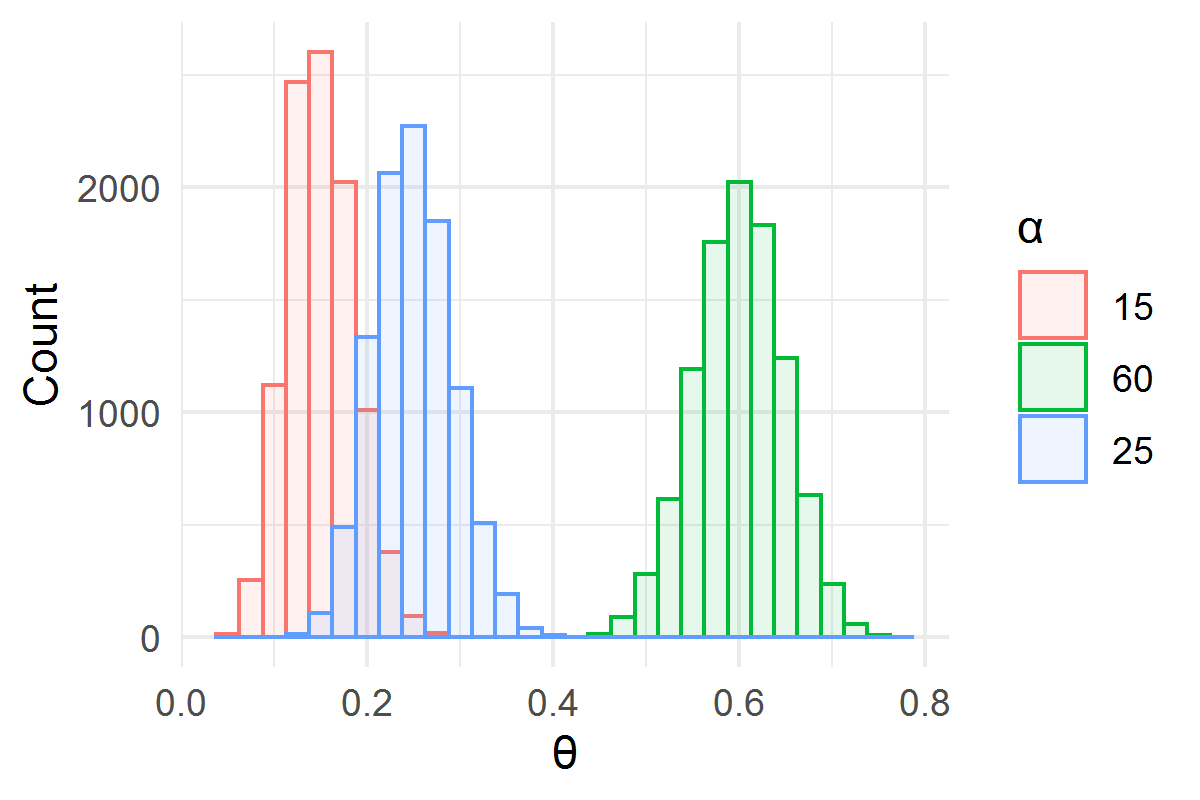
\includegraphics[width=6cm,height=4cm]{figures/DirchletSamples1} \end{center}

This is similar to the shift of the beta distribution when using
hyperparameters that are unequal.

\end{frame}

\begin{frame}{Dirichlet - Multinomial}
\protect\hypertarget{dirichlet---multinomial}{}

\footnotesize

The multinomial distribution with parameters
\(\overrightarrow{\theta} = \theta_{1}, \theta_{2}, ... \theta_{n}\) for
words \(1\) to \(n\) would be capable of generating a bag of words (BOW)
representation of a document. The model will be used to generate a
document using a limited vocabulary, only 3 distinct words:
\(\color{blue} \Theta, \color{red} \Omega, \color{darkgreen} \Psi\)., in
particular using the word counts as our \(\alpha\) values for the
dirichlet prior. \(\color{blue} \Delta\) \(\color{blue} \Delta\)
\(\color{blue} \Delta\) \(\color{blue} \Delta\) \(\color{blue} \Delta\)
\(\color{blue} \Delta\) \(\color{blue} \Delta\) \(\color{blue} \Delta\)
\(\color{red} \Omega\) \(\color{darkgreen} \Psi\)

Then we use the \(\theta\) values generated by the dirichlet prior as
the parameters for a multinomial distribution to generate the next term
in the document.

1 \(\color{blue} \Delta\) \(\color{blue} \Delta\)
\(\color{blue} \Delta\) \(\color{blue} \Delta\) \(\color{blue} \Delta\)
\(\color{blue} \Delta\) \(\color{blue} \Delta\)
\(\color{darkgreen} \Psi\) \(\color{blue} \Delta\)
\(\color{darkgreen} \Psi\) \newline2 \(\color{blue} \Delta\)
\(\color{red} \Omega\) \(\color{blue} \Delta\) \(\color{blue} \Delta\)
\(\color{blue} \Delta\) \(\color{red} \Omega\) \(\color{blue} \Delta\)
\(\color{blue} \Delta\) \(\color{blue} \Delta\) \(\color{red} \Omega\)
\newline3 \(\color{blue} \Delta\) \(\color{blue} \Delta\)
\(\color{blue} \Delta\) \(\color{blue} \Delta\)
\(\color{darkgreen} \Psi\) \(\color{blue} \Delta\)
\(\color{red} \Omega\) \(\color{darkgreen} \Psi\)
\(\color{blue} \Delta\) \(\color{blue} \Delta\) \newline4
\(\color{blue} \Delta\) \(\color{red} \Omega\) \(\color{blue} \Delta\)
\(\color{red} \Omega\) \(\color{blue} \Delta\) \(\color{red} \Omega\)
\(\color{blue} \Delta\) \(\color{blue} \Delta\) \(\color{blue} \Delta\)
\(\color{blue} \Delta\) \newline5 \(\color{blue} \Delta\)
\(\color{blue} \Delta\) \(\color{blue} \Delta\) \(\color{blue} \Delta\)
\(\color{red} \Omega\) \(\color{blue} \Delta\) \(\color{blue} \Delta\)
\(\color{darkgreen} \Psi\) \(\color{blue} \Delta\)
\(\color{blue} \Delta\) \newline

\end{frame}

\begin{frame}{Inference I}
\protect\hypertarget{inference-i}{}

\footnotesize

The process above is a \textbf{generative model}. Now we are going to
take a series of pre-existing documents and infer what model created
them

Once we plug in the prior and likelihood and simplify, we find that we
are left with a Dirichlet PDF with the input parameters of
\(\overrightarrow{\alpha} + \overrightarrow{n}\) where \emph{n} are the
observed word counts.

\begin{equation}
\begin{aligned}
p(\theta|D) &\propto p(D|\theta)p(\theta)\\
&\propto \prod _{i=1}^{K}\theta^{n(k)} { 
  {\Gamma {\bigl (}\sum _{i=1}^{K}\alpha _{i}{\bigr )}}
  \over{\prod _{i=1}^{K}\Gamma (\alpha _{i})}
}
\prod _{i=1}^{K}\theta_{i}^{\alpha _{i}-1} \\
&\propto{ 
  {\Gamma {\bigl (}\sum _{i=1}^{K}\alpha _{i}{\bigr )}}
  \over{\prod _{i=1}^{K}\Gamma (\alpha _{i})}
}\prod _{i=1}^{K}\theta_{i}^{\alpha _{i}+n_{k}-1} \\
&\propto Dir(\overrightarrow{\alpha} + \overrightarrow{n})
\end{aligned}
\end{equation}

\end{frame}

\begin{frame}{Inference II}
\protect\hypertarget{inference-ii}{}

Let's use the 5 documents we previously generated as our basis and infer
the parameters used to generate them via Gibbs sampling.

\begin{center}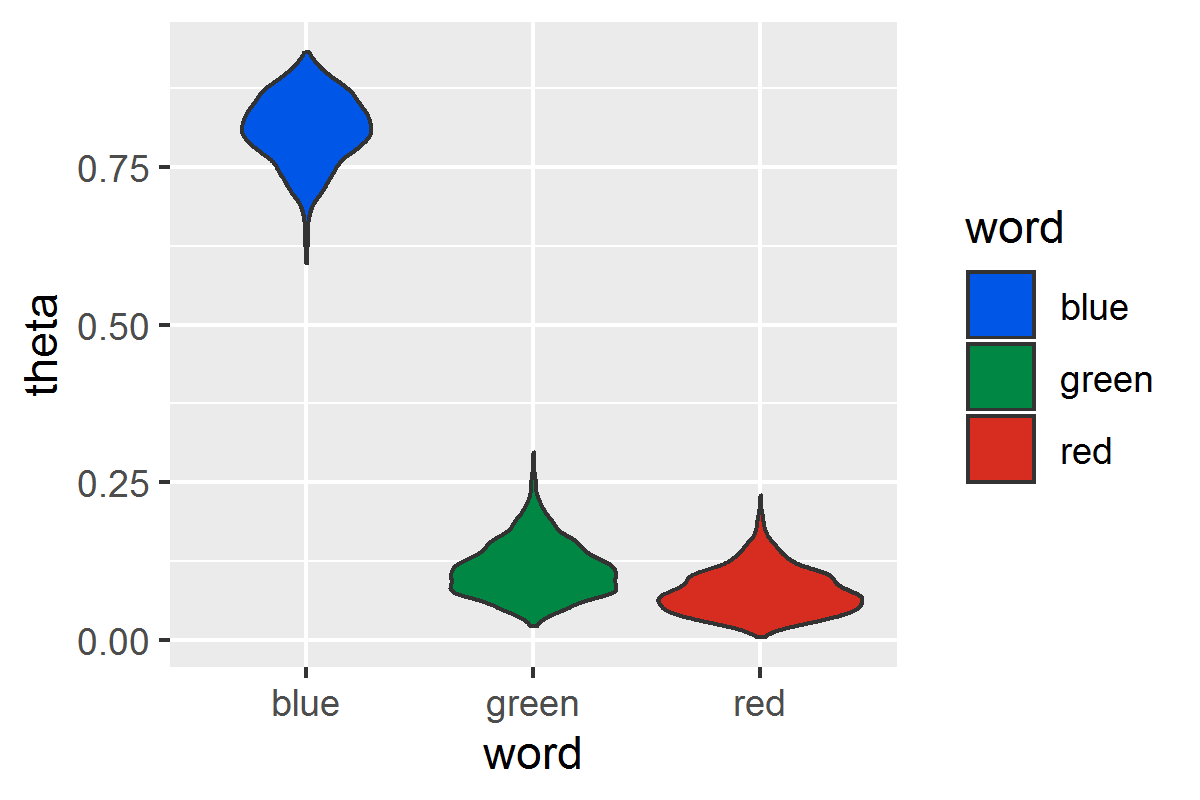
\includegraphics[width=8cm,height=6cm]{figures/unigramInference10} \end{center}

\end{frame}

\begin{frame}{Inference III}
\protect\hypertarget{inference-iii}{}

Instead of just 5 documents we will generate 500 and use this as our
sample to infer the word mixtures from.

\begin{center}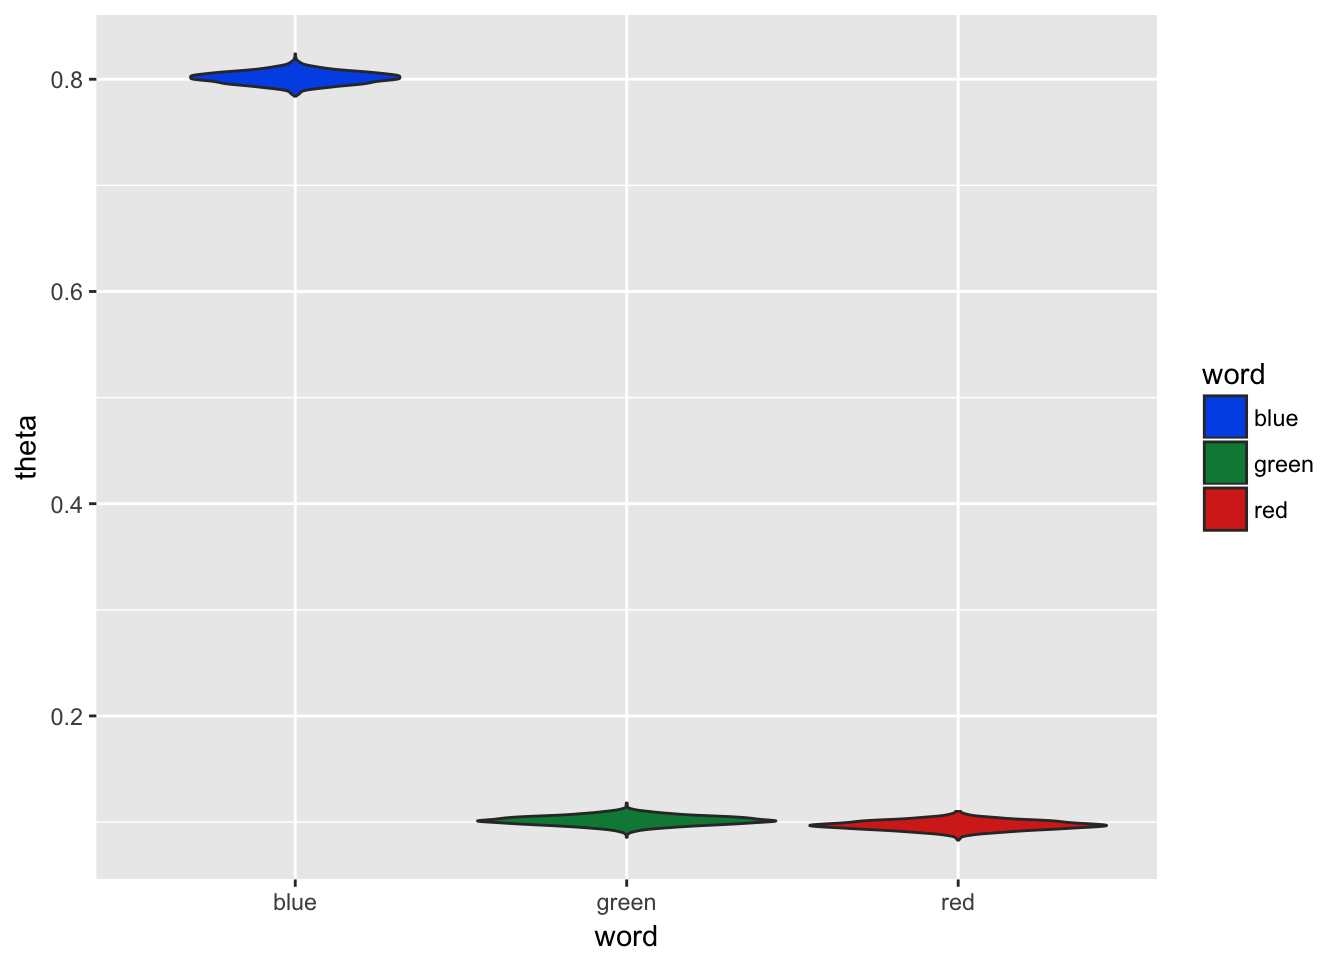
\includegraphics[width=8cm,height=6cm]{figures/unigramInference500} \end{center}

\end{frame}

\begin{frame}{Mixture of Words \textbf{and} Topics}
\protect\hypertarget{mixture-of-words-and-topics}{}

\footnotesize

\begin{itemize}
\tightlist
\item
  \textbf{Documents (d in D):}, that we want to identify the topic
  structures of.
\item
  \textbf{Words (w in W):} We have a collection of words and word counts
  for each document.
\item
  \textbf{Hyperparameters:}

  \begin{itemize}
  \tightlist
  \item
    \(\overrightarrow{\alpha}\): Our prior assumption about the topic
    distribution of our documents. We will be supplying the \(\alpha\)
    value for inference.

    \begin{itemize}
    \tightlist
    \item
      Higher \(\overrightarrow{\alpha}\) - We assume documents will have
      a similar and close to uniform distribution of topics.
    \item
      Lower \(\overrightarrow{\alpha}\) - We assume document topic
      distributions vary more drastically.
    \end{itemize}
  \item
    \(\overrightarrow{\beta}\): Our prior assumption about the word
    distribution of each topic.

    \begin{itemize}
    \tightlist
    \item
      Higher \(\overrightarrow{\beta}\): Word distributions in each
      topic are closer to uniform, i.e.~each word is equally as likely
      in each topic.
    \item
      Lower \(\overrightarrow{\beta}\): Word distributions vary more
      from topic to topic.
    \end{itemize}
  \end{itemize}
\end{itemize}

\end{frame}

\begin{frame}{Latent Dirichlet allocation}
\protect\hypertarget{latent-dirichlet-allocation}{}

\footnotesize

Latent Dirichlet allocation is one of the most common algorithms for
topic modeling. It is guided by two principles.

\begin{itemize}
\tightlist
\item
  \textbf{Every document is a mixture of topics.} We imagine that each
  document may contain words from several topics in particular
  proportions. For example, in a two-topic model we could say ``Document
  1 is 90\% topic A and 10\% topic B, while Document 2 is 30\% topic A
  and 70\% topic B.''
\item
  \textbf{Every topic is a mixture of words.} For example, we could
  imagine a two-topic model of American news, with one topic for
  ``politics'' and one for ``entertainment.'' The most common words in
  the politics topic might be ``President'', ``Congress'', and
  ``government'', while the entertainment topic may be made up of words
  such as ``movies'', ``television'', and ``actor''. Importantly, words
  can be shared between topics; a word like ``budget'' might appear in
  both equally.
\end{itemize}

\end{frame}

\begin{frame}{Simplified View}
\protect\hypertarget{simplified-view}{}

\begin{itemize}
\item Go through each document $d$, and randomly assign each word in the document to one of the $K$ topics.
\item For each document $d$, 
   \begin{itemize}
      \item For each word $w$ in $d$, and each topic $t$, compute: 
      \begin{enumerate}
        \item $p( t |  d)$ =  proportion of words in document $d$ that are currently assigned to topic $t$, and        
        \item $p( w |  t)$ =  proportion of assignments to topic $t$ over all documents that come from this word $w$.
        \item Reassign $w$ a new topic $t$ with the probability that topic $t$ generated word $w$: $p( t |  d) \cdot p( w |  t)$
      \end{enumerate}
    \end{itemize}   
\end{itemize}

In the last step, we're assuming that all topic assignments except for
the current word in question are correct, and then updating the
assignment of the current word using our model of how documents are
generated.

\end{frame}

\begin{frame}{Gibbs Sampling}
\protect\hypertarget{gibbs-sampling}{}

The main goal of inference in LDA is to determine the topic of each word
\(w\), \(z_{i}\) (topic of word \emph{i}), in each document:
\(p(z_{i}|z_{\neg i}, \alpha, \beta, w)\).

\begin{equation}
\begin{aligned}
p(z_{i}|z_{\neg i}, w) & \propto {n_{d,\neg i}^{k} + \alpha_{k} \over 
  \sum_{k} n_{d,\neg i}^{k} + \alpha_{k}} \cdot {n_{k,\neg i}^{w} + \beta_{w} \over 
  \sum_{w} n_{k,\neg i}^{w} + \beta_{w}}
\end{aligned}
\end{equation}

where

\begin{itemize}
\item
  \(n_{d,\neg i}^{k}\): Number of times document \(d\) use topic \(k\)
\item
  \(n_{k,\neg i}^{w}\): Number of times topic k uses the given word
\end{itemize}

\end{frame}

\end{document}
